\chapter{\label{ch1-intro}Introduction} 

\minitoc

\section{Atmospheric Cherenkov Showers}

\begin{figure}
  \begin{subfigure}[b]{0.49\textwidth}
    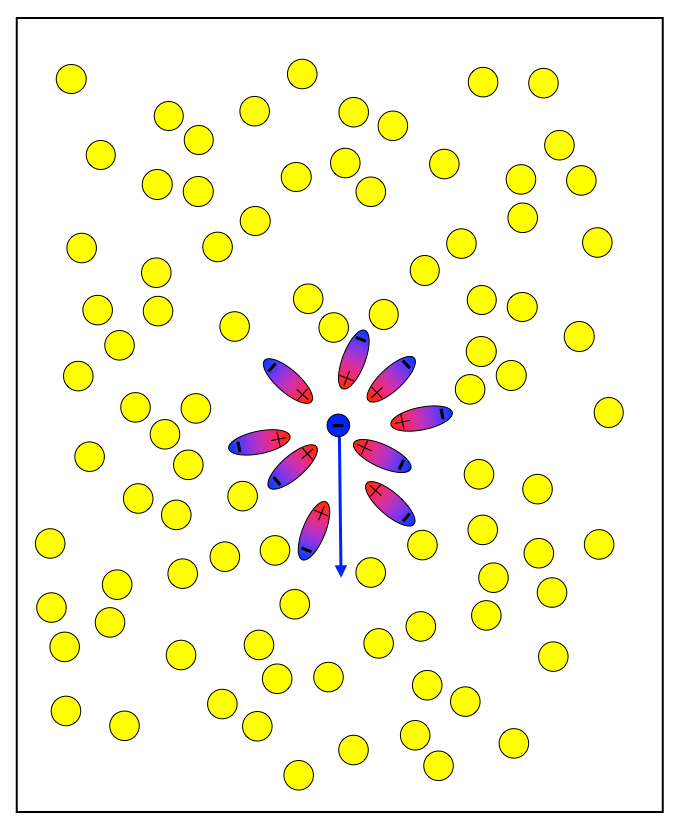
\includegraphics[width=\textwidth]{dipole_slow}
    \caption{$v < \frac{c}{n}$}
    \label{fig:dipole_slow}
  \end{subfigure}
  \hfill
  \begin{subfigure}[b]{0.49\textwidth}
    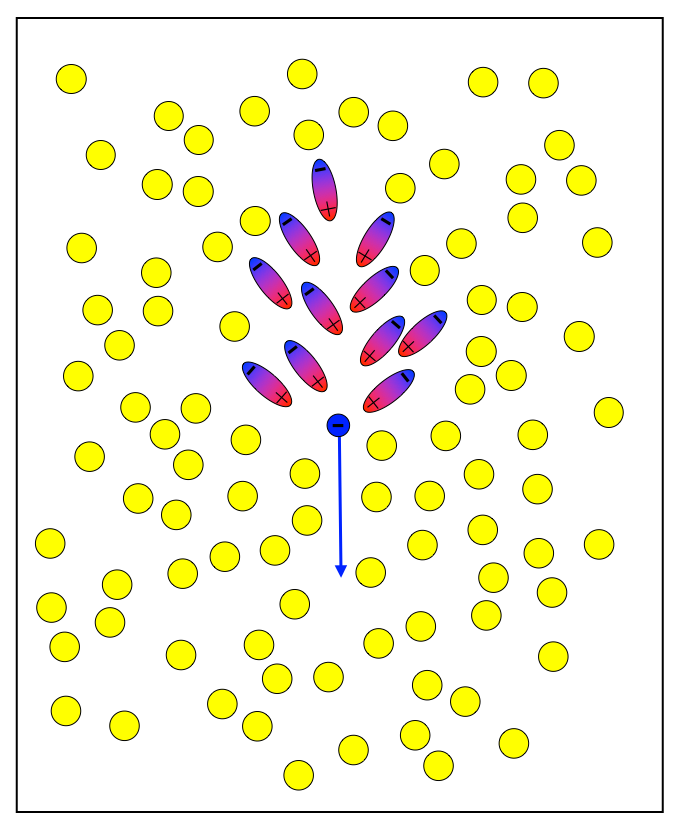
\includegraphics[width=\textwidth]{dipole_fast}
    \caption{$v \ge \frac{c}{n}$}
    \label{fig:dipole_fast}
  \end{subfigure}
  \caption[Polarisation produced in a dielectric medium due to the presence of a charged particle.]{Polarisation produced in a dielectric medium due to the presence of a charged particle, for the cases of a subluminal and superluminal particle.}
\end{figure}

\begin{figure}
	\centering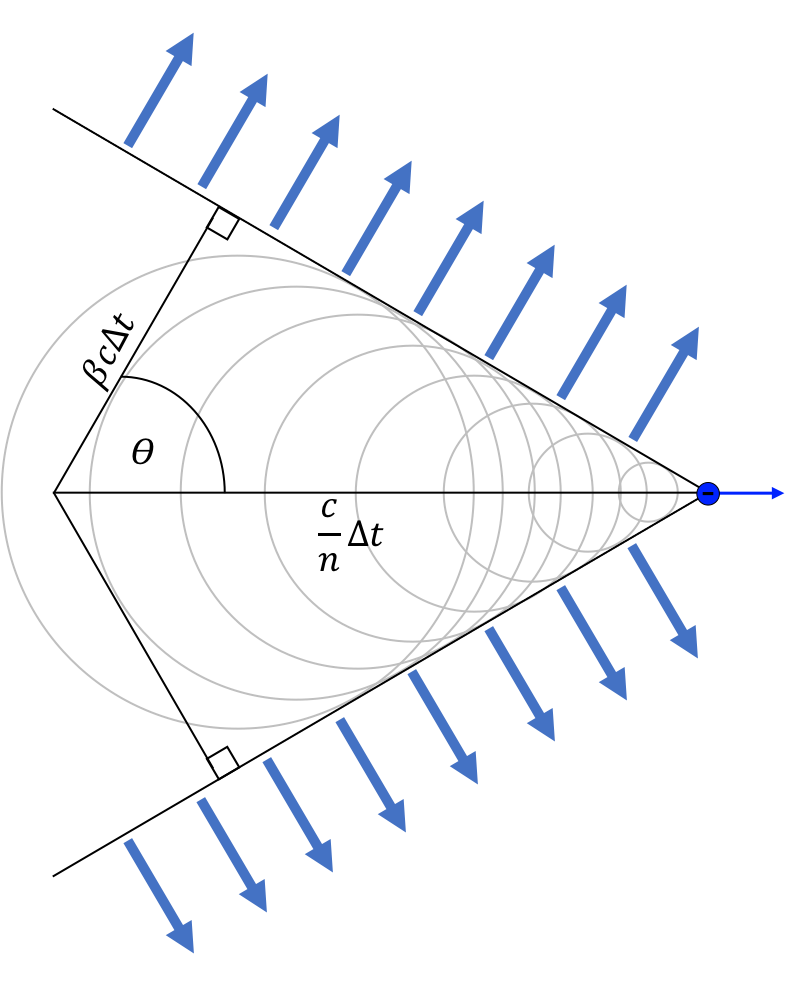
\includegraphics[width=\textwidth]{cherenkov_geom} 
	\caption[Geometry of the wavefronts involved in Cherenkov radiation production.]{Geometry of the wavefronts involved in Cherenkov radiation production. The particle travels at a speed faster than the wavefronts propagate.}
	\label{fig:cherenkov_geom}
\end{figure}

When a charged particle moves slowly through a dielectric medium, the electric field of the particle distorts the nearby atoms. Momentarily, these atoms are transformed into elementary dipoles where the charged particles that constitute the atom are arranged with respect to the electric field of the travelling particle (Figure~\ref{fig:dipole_slow}). Due to the complete symmetry of this polarisation around the travelling particle, no net field is produced by the dielectric medium. However, if instead the velocity of the charged particle is faster than the speed light travels in that medium, an asymmetry along the particle trajectory is formed in the polarisation of the surrounding atoms (Figure~\ref{fig:dipole_fast}), resulting in a net dipole field. As the particle continues through the medium, elements of the polarised medium will release a brief burst of electromagnetic radiation. Generally these electromagnetic waves interfere destructively, except inside in the forward direction along the particles trajectory in an opening angle $\theta$. Although the full characterisation of this relativistic effect is complex, a simple consideration of the geometry involved, shown in Figure~\ref{fig:cherenkov_geom}, can be used to describe $\theta$. In a time $\Delta t$ a particle travels a distance $\beta c \Delta t$ where $\beta = \frac{v}{c}$, while the emitted light will travel a distance $\frac{c}{n} \Delta t$ in a medium with refractive index $n$. This results in the relation:
\begin{equation} \label{eq:cherenkov_angle}
\cos \theta = \frac{c}{vn}.
\end{equation}
The radiation emitted in this constrained opening angle via this phenomena is known as Cherenkov radiation.

A very high energy gamma ray entering the Earth's atmosphere 




($\frac{\text{velocity}}{\text{speed of light}} > \frac{1}{refractive index}$), the  

relativistic particles travel through 




- travel of photons

\section{Imaging Atmospheric Cherenkov Telescopes}

- technique, nsb, trigger curve
- aim of optics, large fov
- time gradient
- history, previous ones
- latest is cta

\section{The Cherenkov Telescope Array}

- Improvements on previous
- Sensitivity
- Energy res?
- angular res?
- Array layout
- LSTs, MSTs, SSTs, and what there purpose is (large mirror area versus large collection area...) 

\section{Small Sized Telecopes}

- Science with ssts
- Three designs

\section{Gamma-ray Cherenkov Telescope}

- what makes us better - lightweight telescope, full waveform readout
- optics








\notes[inline,caption={}]{
	\section{Plan}
	\subsection{Topics}
	\begin{itemize}
		\item High Energy Astrophysics
		\begin{itemize}
			\item Fermi
			\item Fermi Bubbles
			\item HAWC
		\end{itemize}
		\item IACTs
		\item CTA
		\item CTA Science
		\begin{itemize}
			\item Science Cases
			\item Use "Science with CTA" paper
		\end{itemize}
		\item SSTs
		\item SST Science
		\begin{itemize}
			\item What do we contribute?
			\item What can't be done without us?
		\end{itemize}
		\item GCT
		\item CHEC
		\begin{itemize}
			\item What makes us better?
			\item Advantages of Schwarzchild-Couder
			\begin{itemize}
				\item Increased FoV
				\item Size
				\item Cost
			\end{itemize}
			\item Advantages of full waveform readout
			\item Other Advantages?
			\begin{itemize}
				\item Trigger
				\item Energy/power/voltage Requirements
				\item Commonalities (SCT)
			\end{itemize}
		\end{itemize}
	\end{itemize}
	\subsection{Questions}
	\begin{itemize}
		\item ?
	\end{itemize}
}

\change[inline]{Shower properties, photons from bottom of shower are received before those at the top as the particle travels faster than light. Good figure in \cite{Cogan2006}}
\change[inline]{Gamma/Hadron/Lepton}

\change[inline]{Terminology note: charge not used in terms of columns, it refers to counts of photoelectrons, for which mV and ADC are a proxy of. Do a ctrl-f at end to check how charge is used}

\change[inline]{trigger efficiency???}

\change[inline]{introduce SC optics with reference to "modern iteration for utilisation in Cherenkov shower described by \cite{Vassiliev2007}" Giro2017}

low number of photons above 50 TeV, very low, frontier

\section{Atmospheric Cherenkov Showers}

\section{Imaging Atmospheric Cherenkov Technique}

\subsection{Cherenkov Shower Characteristics}

\subsection{Photon Arrival Time} \label{section:photon_arrival_time}

\change[inline]{Quoted from Holder2005: The longitudinal development of an air shower is reflected in the long axis of the elliptical image recorded in the camera. The photon arrival time profile along this axis is largely a result of geometrical path length differences, and hence the shower core distance. As the shower particles move faster than the speed of light in air, when the shower has a small core distance Cherenkov light emitted from lower in the atmosphere is received at the telescope first. At large core distances, this situation is reversed, as the Cherenkov light travel time from the shower to the telescope dominates. The effect of this is to produce a timing gradient along the long axis of the image, the size and sign of which depend upon the core distance. For gamma-ray showers from a point source at the centre of the field of view, the shower core distance is directly related to the angular distance in the camera of the image from the source position.
Figure}

\section{The Cherenkov Telescope Array}

CTA will be, for the first time in VHE gamma-ray astronomy, operated as an open observatory.

\section{Small Sized Telescopes}

\section{Science with the Small Sized Telescopes}

